\documentclass[a4paper,12pt]{article}
\usepackage[a4paper,top=1.3cm,bottom=2cm,left=1.5cm,right=1.5cm,marginparwidth=0.75cm]{geometry}

% Пакеты
\usepackage{mathtext} 
\usepackage{setspace}
\usepackage{tabularx}
\usepackage{cmap}
\usepackage{longtable}
\usepackage{icomma}
\usepackage{euscript}
\usepackage{float}
\usepackage{cutwin}
\usepackage{mathrsfs}
\usepackage{adjustbox}
\usepackage{dashbox}
\usepackage[normalem]{ulem}
\usepackage[T2A]{fontenc}			
\usepackage[utf8]{inputenc}                 %!  закрепляет кодировку utf8
\usepackage[english,russian]{babel}         %!  подключает русский и английский
%математические шрифты:
\usepackage{amsmath,amsfonts,amssymb,amsthm,mathrsfs,mathtools} 
\usepackage[colorlinks, linkcolor = purple]{hyperref}      %!  оглавление для панели навигации по PDF-документу + гиперссылки
\usepackage{xcolor}                         %!  добавляет цвета
\usepackage{enumitem}                       %!  задание макета перечня.
\usepackage{xpatch}                         %?  работа с renewcommand и макросами              
\usepackage{cancel}                         %   зачёкивания текста (!!!) для slash-нотации использовать \usepackage{slashed}!!
\usepackage{upgreek}                        %   заглавные греческие буквы
\usepackage{lipsum}                         %?  для вставки кучи текста при форматировании
\usepackage[version=4]{mhchem}              %   химические формулы
\usepackage{multirow}                       %   объединение строк в матрицах
\usepackage{stackengine}                    %   stack символов
\usepackage{tikz}                           %!  рисунки
\usetikzlibrary{positioning}                %?  библиотека для тикза 
\usepackage{titletoc}                       %!  форматирование содержания и заголовков
\usepackage{titlesec}                       %!  форматирование содержания и заголовков
\usepackage{wrapfig}                        %   обтекание таблиц и рисунков
\usepackage{chngcntr}                       %!  для setcounter
\usepackage{fancyhdr}                       %!  для колонтитулов
\usepackage{makecell}                       %?  матрицы с разными выравниваниями и т.п
\usepackage{indentfirst}                    %   добавить indent перед первым 
\usepackage{tocloft}                        %?  изменение названий глав и разделов                       
\usepackage{soul}                           %   типографические примочки, типо зачёркивания и подчёркивания
\usepackage[stable]{footmisc}               %?  продвинутые сноски
\usepackage{subfig}                         %   несколько картинок рядом
   %  задаёт поля страниц

% pgf plots
% \usepackage{pgfplots}
% \pgfplotsset{compat=1.17}

\mathtoolsset{showonlyrefs=true}

%Обозначения теорем и т.п
\theoremstyle{definition}
\newtheorem*{definition}{Определение}
\newtheorem{statement}{Предложение}[section]
\newtheorem{lemma}{Лемма}[section]
\newtheorem{theorem}{Теорема}[section]
\newtheorem*{theoremn}{Теорема}
\newtheorem*{corollary}{Следствие}
\newtheorem*{example}{Пример}
\newtheorem*{note}{Замечание}
\newtheorem*{problem}{Задача}

%Шарабара для содержания и внешнего вида нумерации
\counterwithout{footnote}{section}\DeclareRobustCommand{\divby}{%
	\mathrel{\text{\vbox{\baselineskip.65ex\lineskiplimit0pt\hbox{.}\hbox{.}\hbox{.}}}}%
}

\usepackage{titlesec}
\titlelabel{\thetitle.\quad} %точка в section

%Толерантный квадратик чтд
%\makeatletter \renewenvironment{proof}[1][\proofname]{\par\pushQED{\qed}\normalfont\topsep6\p@\@plus6\p@\relax\trivlist\item[\hskip\labelsep\bfseries#1\@addpunct{.}]\ignorespaces}{\popQED\endtrivlist\@endpefalse} \makeatother
%\renewcommand\qedsymbol{$\squareulblack$}
%\newcommand{\usubseteq}{\mathbin{\rotatebox[origin=c]{90}{$\subset$}}}
%\DeclareFontEncoding{LS2}{}{\noaccents@}
%\DeclareFontSubstitution{LS2}{stix}{m}{n}
%\DeclareSymbolFont{arrows3}{LS2}{stixtt}{m}{n}
%\DeclareMathSymbol{\squareulblack}{\mathord}{arrows3}{"88}

%Разные операторы и символы
\newcommand{\dotpr}[2]{\bra{#1}\ket{#2}}
\let\AA\relax
%\let\oldvarphi\phi %оно делает так, что \phi становится правильным фи
%\let\phi\varphi
%\let\varphi\oldvarphi
\let\emptyset\varnothing
\DeclareMathOperator*{\esssup}{ess sup}
\DeclareMathOperator*{\ord}{ord}
\DeclareMathOperator*{\supp}{supp}
\DeclareMathOperator*{\pr}{pr}
\DeclareMathOperator*{\Ker}{Ker}
\DeclareMathOperator*{\Vol}{Vol}
\DeclareMathOperator*{\rg}{rk}
\DeclareMathOperator*{\Ima}{Im}
\DeclareMathOperator*{\Alt}{Alt}
\DeclareMathOperator*{\Sym}{Sym}
\newcommand{\eqdef}{\stackrel{\text{\tiny{def}}}{=}}
\newcommand{\pp}{\partial}
\newcommand{\AA}{\mathcal{A}}
\newcommand{\BB}{\mathcal{B}}
\newcommand{\MM}{\mathbb{M}}
\newcommand{\NN}{\mathbb{N}}
\newcommand{\ZZ}{\mathbb{Z}}
\newcommand{\QQ}{\mathbb{Q}}
\newcommand{\RR}{\mathbb{R}}
\newcommand{\CC}{\mathbb{C}}
\newcommand{\FFF}{\mathbb{F}}
\newcommand{\DD}{\mathcal{D}}
\newcommand{\FF}{\mathcal{F}}
\newcommand{\sS}{\mathcal{S}}
\newcommand*\circled[1]{\tikz[baseline=(char.base)]{
		\node[shape=circle,draw,inner sep=2pt] (char) {#1};}}


%%% Заголовок
\author{Шерхалов Денис Б02-204}
\title{Лабораторная работа 2.2.1 \\
	\textbf{Исследование взаимной диффузии газов}}
\date{\today}

\begin{document}
	
	{\Large \maketitle}
	
	\paragraph*{Цель работы:} 1) регистрация зависимости концентрации гелия в воздухе от времени с помощью датчиков теплопроводности при разных начальных давлениях смеси газов; 2) определение коэффициента диффузии по результатам измерений.
	
	\paragraph*{В работе используются:} измерительная установка; форвакуумный насос; баллон с газом  (гелий); манометр; источник питания; магазин сопротивлений; гальванометр; секундомер.
	
	\section{Введение}
	
	\textit{Диффузией} называют самопроизвольное взаимное проникновение веществ друг в друга, происходящее вследствие хаотичного теплового движения молекул. При перемешивании молекул разного сорта говорят о взаимной (или концентрационной) диффузии.
	
	Диффузия в системе, состоящей из двух компонентов $ a $ и $ b $ (бинарная смесь), подчиняется закону Фика: плотности потока компонентов $ j_{a,b} $ (количество частиц, пересекающих единичную площадку в единицу времени) пропорциональны градиентам их концентраций $ \nabla n_{a,b}$, что в одномерном случае можно записать как
	
	\[ j_a = -D\dfrac{\partial n_a}{\partial x}, \quad j_b = -D\dfrac{\partial n_b}{\partial x}, \]
	где $ D $ -- коэффициент взаимной диффузии компонентов. Знак <<минус>> отражает тот факт, что диффузия идёт в направлении выравнивания концентраций. Равновесие достигается при равномерном распределении вещества по объёму сосуда ($ \partial n / \partial x = 0 $).
	
	В случае работы с данной установкой можно считать, что диффузионный поток одинаков в любом сечении трубки, соединяющей сосуды $V_1$ и $V_2$. Следовательно:
	
	\begin{align}
		J = -DS\dfrac{n_1-n_2}{l} \qquad DS\frac{n_1-n_2}{l} = -V_1\dfrac{dn_1}{dt} = V_2\dfrac{dn_2}{dt} \\
		\dfrac{dn_1 - dn_2}{dt} = -\dfrac{n_1-n_2}{l}DS\left(\dfrac{1}{V_1}+\dfrac{1}{V_2}\right) \quad\Rightarrow\quad n_1-n_2 = (n_1-n_2)_0 e^{-\frac{t}{\tau}}
	\end{align}
	
	В данной работе исследуется взаимная диффузия гелия и воздуха. Давление P и температура T в условиях опыта предполагаются неизменными: $ p=(n_{He}+n_{\text{в}})kT $, где $ n_{He} $ и $ n_{\text{в}} $ -- концентрации (объёмные плотности) диффундирующих газов. Поэтому для любых изменений концентраций справедливо $ \Delta n_{He}=-\Delta n_{\text{в}} $. Следовательно, достаточно ограничиться описанием диффузии одного из компонентов, например гелия $ n_{He} $:
	
	\begin{equation}\label{1}
		j_{He}=-D\dfrac{\partial 	n_{He}}{\partial x}.
	\end{equation}
	
	Приведём теоретическую оценку для коэффициента диффузии. В работе концентрация гелия, как правило, мала $ (n_{He} \ll n_\text{в}) $. Кроме того, атомы гелия существенно легче молекул, составляющих воздух ($ \mu_{He} \ll \mu_{O_2}, \mu_{N_2} $), значит и их средняя тепловая скорость велика по сравнению с остальными частицами. Поэтому перемешивание газов в работе можно приближенно описывать как диффузию примеси лёгких частиц $ He $ на практически стационарном фоне воздуха. Коэффициент диффузии в таком приближении равен
	
	\begin{equation}\label{2}
		D=\dfrac{1}{3}\lambda 	\overline{v},
	\end{equation}
	
	где $ \overline{v}=\sqrt{\frac{8RT}{\pi \mu}} $ -- средняя тепловая скорость частиц примеси, $ \lambda = \frac{1}{n_0\sigma} $ -- их длина свободного пробега, $ n_0 $ -- концентрация рассеивающих центров (фона), $ \sigma $ -- сечение столкновения частиц примеси с частицами фона.
	
	Таким образом, теория предсказывает, что коэффициент диффузии бинарной смеси обратно пропорционален давлению в системе $ D \propto 1/P $, и не зависит от пропорций компонентов, что и предлагается проверить в работе экспериментально.
	
	\subsection*{Экспериментальная установка}
	
	\begin{wrapfigure}{l}{7.25cm}
		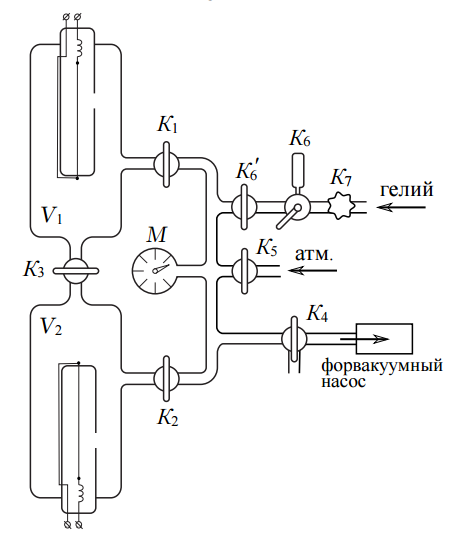
\includegraphics[scale=0.8]{facility}				
		\caption{Схема установки}
		\label{facility}
	\end{wrapfigure}
	Для исследования взаимной диффузии используется следующая установка:
	
	Здесь $V_1,\; V_2$ -- два сосуда с примерно равным объемом, в которые мы будем загонять воздух и гелий.
	
	Данная конструкция позволяет провести диффузию, которая возможна только при равенстве давлений.
	
	Основное оборудование, с помощью которого мы будем снимать измерения -- датчики теплопроводности, через которые пропускают ток. Они подключены к мосту, который позволяет нам устанавливать начальное равновесное состояние.
	
	При изменении концентрации в колбах вольтметр покажет нам разность напряжений на датчиках, что, из-за их конструкции, означает разность концентраций. 
	
	С помощью изменения напряжения мы и будем изучать процесс диффузии, т.к. во время ее протекания концентрации газов начинают устанавливаться, что заметно на графике разницы напряжений от времени.
	
	\section{Выполнение}
		
		\begin{enumerate}
			\item Ознакомимся с установкой. Наша установка -- 1.
			
			\item Для смеси гелий-воздух исследуем зависимость коэффициента взаимной диффузии о начального давления в системе. Для этого будем фиксировать с помощью компьютера в лаборатории зависимость показаний вольтметра от времени, прошедшего с начала эксперимента. Полученные результаты находятся в папке "Санников Шерхалов", и не были продублированы в отчете, т.к. содержат очень много данных. Эксперимент проводился при давлении $P$=753.6торр. 
			
			\item По полученным результатам нарисуем график зависимости логарифма напряжения от времени. Проверим то, что процесс диффузии подчиняется закону: \[U = (U)_0e^{-\dfrac{t}{\tau}}.\]
			
			
			\begin{figure}[h!]
				\centering
				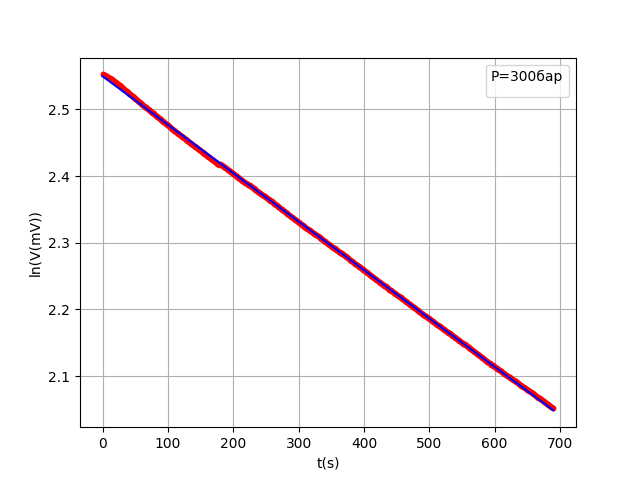
\includegraphics[scale=0.542]{-0.000727.png}
	                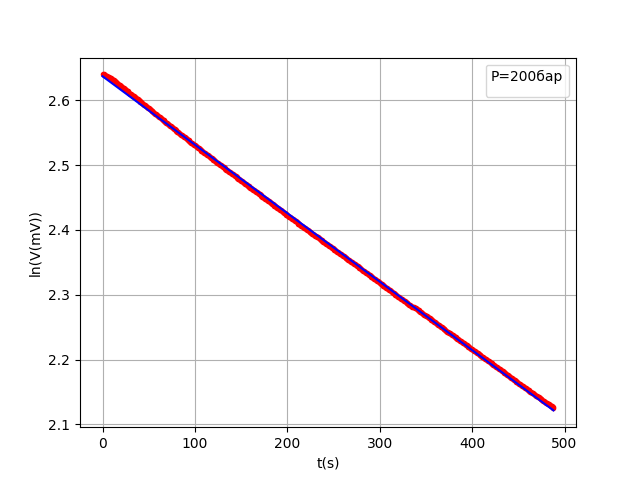
\includegraphics[scale=0.542]{-0.001056.png}
	                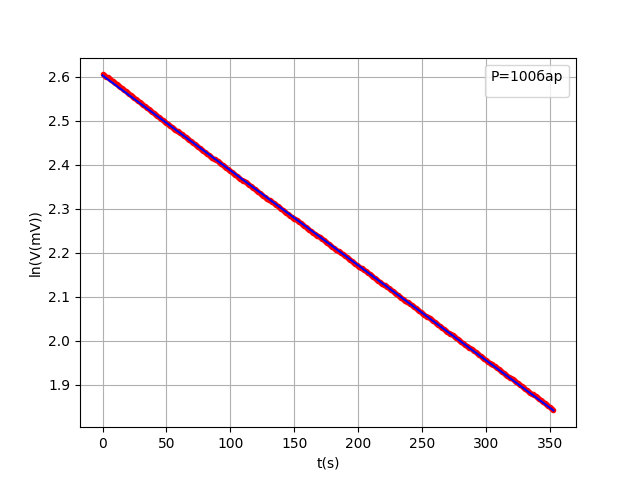
\includegraphics[scale=0.542]{-0.002154.png}
	                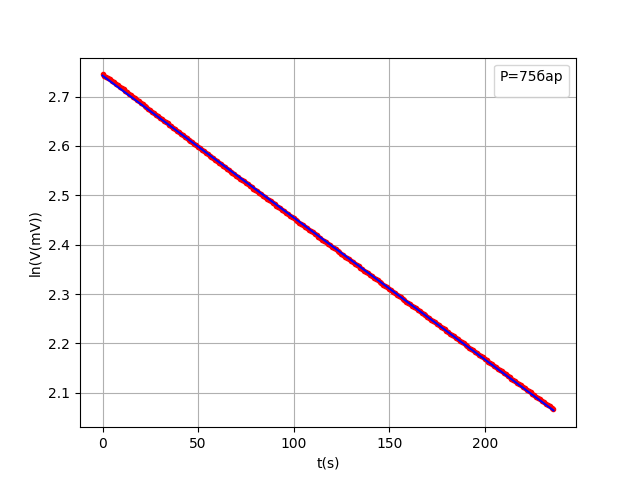
\includegraphics[scale=0.542]{-0.002873.png}
	                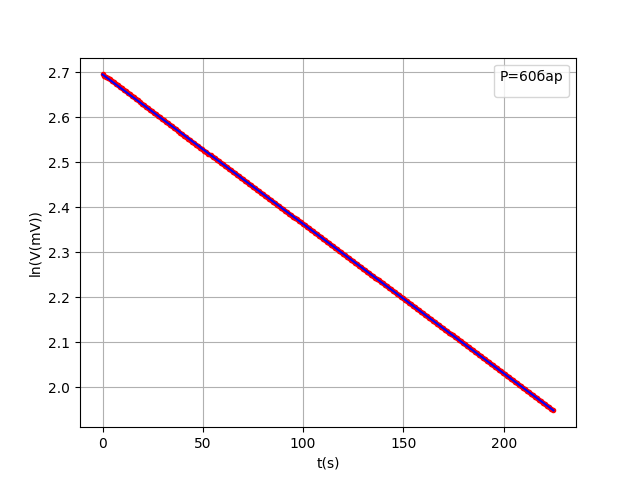
\includegraphics[scale=0.542]{-0.003321.png}
	                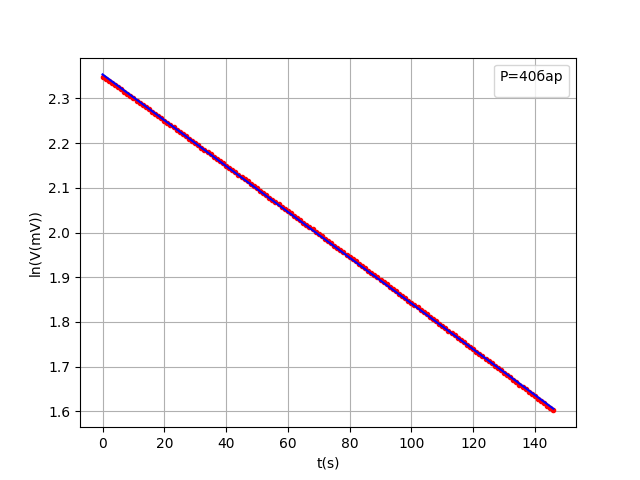
\includegraphics[scale=0.542]{-0.005126.png}
				
			\end{figure}
		
			\item Графики линейны, следовательно у нас действительно происходит диффузия. Далее мы можем найти $\tau$ как коэффициент наклона. Находить будем по МНК. В нашем случае: $$\ln{U} =a - k t \qquad k = \frac{1}{\tau}$$
			
			
			\item Проведем расчеты для каждого значения давления, получим таблицу:
			\bgroup
			\def\arraystretch{1.3}%
			\begin{table}[H]
				\centering
				\begin{tabular}{|c|c|c|}
					\hline
					$ P $, торр &  $ k \cdot 10^{-3} $, с$ ^{-1} $ & $ \tau $, с \\ \hline
					37 & 5.126  & 195 \\ \hline
					63 & 3.321  & 301 \\ \hline
					75 & 2.873  & 348 \\ \hline
					97 & 2.154 & 464 \\ \hline
					201 & 1.056  & 947 \\ \hline
	                    295 & 0.727 &  1376\\ \hline
				\end{tabular}
				
			\end{table}
			\egroup
	            Погрешность $k$ и $\tau$ получилась менее 0.1$\%$, поэтому отдельно она не указана.
	            
	
			\item Далее посчитаем коэффициенты взаимной диффузии для различных давлений по формуле:
		
			$$D = \frac{1}{\tau}\frac{VL}{2S}$$
			$$\Delta D = D \cdot \sqrt{\left(\frac{\Delta \tau}{\tau}\right)^2 + \left(\frac{\Delta V}{V}\right)^2 + \left(\frac{\Delta L}{L}\right)^2 + \left(\frac{\Delta S}{S}\right)^2}$$
	
	  
			Параметры моей установки (1): $V = (775\pm 10)\text{ см}^3$, $\dfrac{L}{S} = (5,3\pm 0,1)\text{ }\dfrac{1}{\text{см}}$. 
			
			Посчитаем $D\text{ и }\Delta D$:
			
			\bgroup
			\def\arraystretch{2}%
			\begin{table}[H]
				\centering
				\begin{tabular}{|c||c|c|c|c|c|c|}
					
					\hline
					$ P $, торр & 37&63&75&97&201 & 295\\
					\hline
					$ D $, $\dfrac{\text{см}^2}{\text{с}}$ & 10.53& 6.82& 5.90 & 4.43 & 2.17 & 1.49\\
					\hline
					$ \Delta D $, $\dfrac{\text{см}^2}{\text{с}}$ & 0.22& 0.14 & 0.12& 0.09&0.04 &0.03\\
					\hline
				\end{tabular}
				\caption{Значения коэффициента диффузии при различных давлениях}
				\label{tab:D}
			\end{table}
			\egroup
			
			\newpage 
			
			\item Построим график зависимости $D\left(\dfrac{1}{P}\right)$:
			
			\begin{figure}[H]
				\centering{
				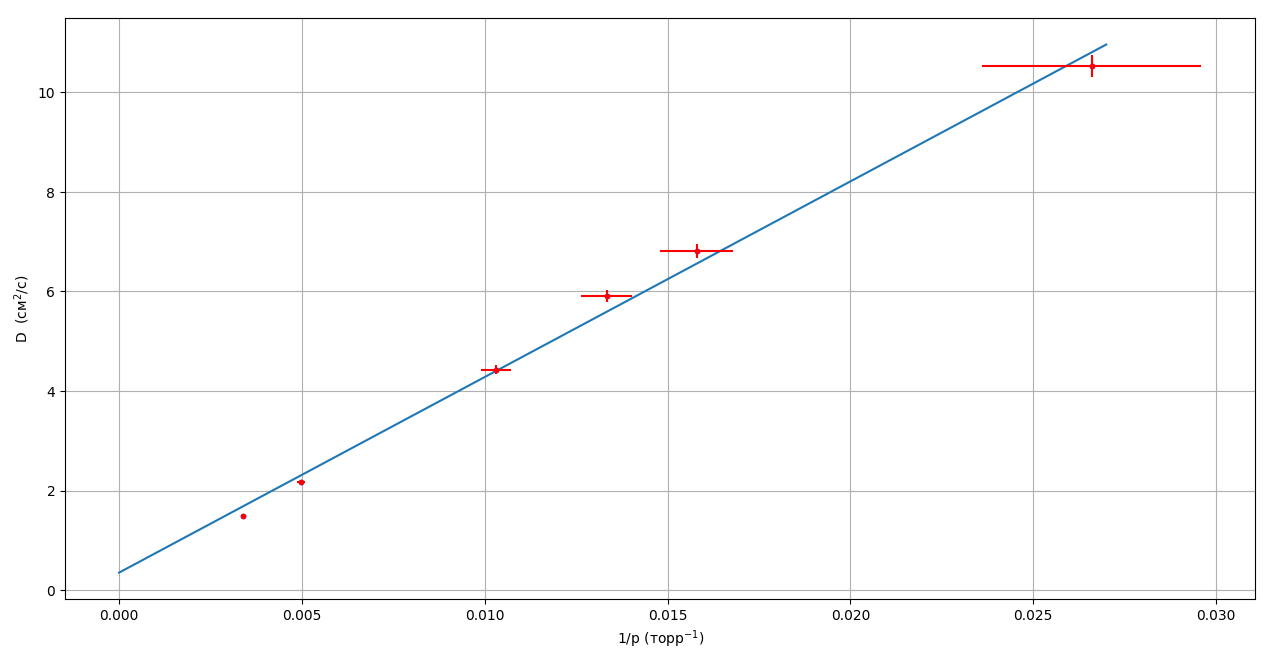
\includegraphics[scale=0.5]{1234.png}
				\caption{Зависимость $ D $ от $ \dfrac{1}{P} $}
				\label{graph2}}
			\end{figure}

			Найдем коэффициент наклона $k = (390\pm10)\text{ } \frac{\text{см}^2}{\text{с}\cdot\text{торр}}$. 
			
			\item Значит, коэффициент диффузии при атмосферном давлении можно найти таким образом:\[D_\text{атм} = k\dfrac{1}{P_\text{атм}} = (0,52\pm0,01)\text{ } \frac{\text{см}^2}{\text{с}}\]
			
			\item По полученным данным оценим длину свободного пробега атомов гелия в воздухе:
			
			\begin{align}
				D=\dfrac{1}{3}\lambda\langle v\rangle,\text{ где } \langle v \rangle = \sqrt{\dfrac{8RT}{\pi \mu}} \Rightarrow \lambda = 3D\sqrt{\dfrac{\pi \mu}{8RT}} \approx 130\text{ нм}
			\end{align}
	
		\end{enumerate}
	
		
	\section{Вывод}
		
		\begin{itemize}
			\item Была зарегистрирована зависимость концентрации гелия в воздухе от времени с помощью датчиков теплопроводности при различных начальных давлениях смеси газов.
			\item По результатам измерений был определен коэффициент взаимной диффузии для смеси гелий-воздух: $D_\text{атм} = (0,52\pm0,01)\text{ } \frac{\text{см}^2}{\text{с}}$ , что близко к табличному значению: $D_\text{табл} = 0,62\text{ } \frac{\text{см}^2}{\text{с}}$. 
			
			\item Была оценена длина свободного пробега гелия в воздухе: $\lambda = (130\pm 3)\text{ нм}$, что близко к табличным данным: $\lambda_\text{табл} = 175\text{ нм}$. 
		\end{itemize}
	
		Основная доля ошибок приходится на барометр и на тот факт, что мост легко расстраивался. Еще метод МНК очень сильно зависит от точки с наибольшей ошибкой, так как если выкинуть ее, и провести те же действия, мы получим D=0.58, что уже ближе к табличному значению.
		
	
\end{document}
